\documentclass[a4paper,12pt]{book} % nie: report!


% pakiety
\usepackage{polski} % lepiej to zamiast babel!
\usepackage[utf8]{inputenc} % w razie kłopotów spróbować: \usepackage[utf8x]{inputenc}
\usepackage{fancyhdr} % nagłówki i stopki
\usepackage{indentfirst} % WAŻNE, MA BYĆ!
\usepackage{lipsum}
\usepackage[pdftex]{graphicx} % to do wstawiania rysunków
\usepackage{amsmath} % to do dodatkowych symboli, przydatne
\usepackage[pdftex,
            left=1in,right=1in,
            top=1in,bottom=1in]{geometry} % marginsy
\usepackage{amssymb} % to też do dodatkowych symboli, też przydatne
\usepackage{pdfpages} % żeby wstawić stronę tytułową
% jesli potrzeb, można oczywiście wstawić inne pakiety i swoje definicje...
  

% definicje nagłówków i stopek
\pagestyle{fancy}
\renewcommand{\chaptermark}[1]{\markboth{#1}{}}
\renewcommand{\sectionmark}[1]{\markright{\thesection\ #1}}
\fancyhf{}
\fancyhead[LE,RO]{\footnotesize\bfseries\thepage}
\fancyhead[LO]{\footnotesize\rightmark}
\fancyhead[RE]{\footnotesize\leftmark}
\renewcommand{\headrulewidth}{0.5pt}
\renewcommand{\footrulewidth}{0pt}
\addtolength{\headheight}{1.5pt}
\fancypagestyle{plain}{\fancyhead{}\cfoot{\footnotesize\bfseries\thepage}\renewcommand{\headrulewidth}{0pt}}

% interlinia
\linespread{1.25}


% treść
\begin{document}
\sloppy



\thispagestyle{empty}

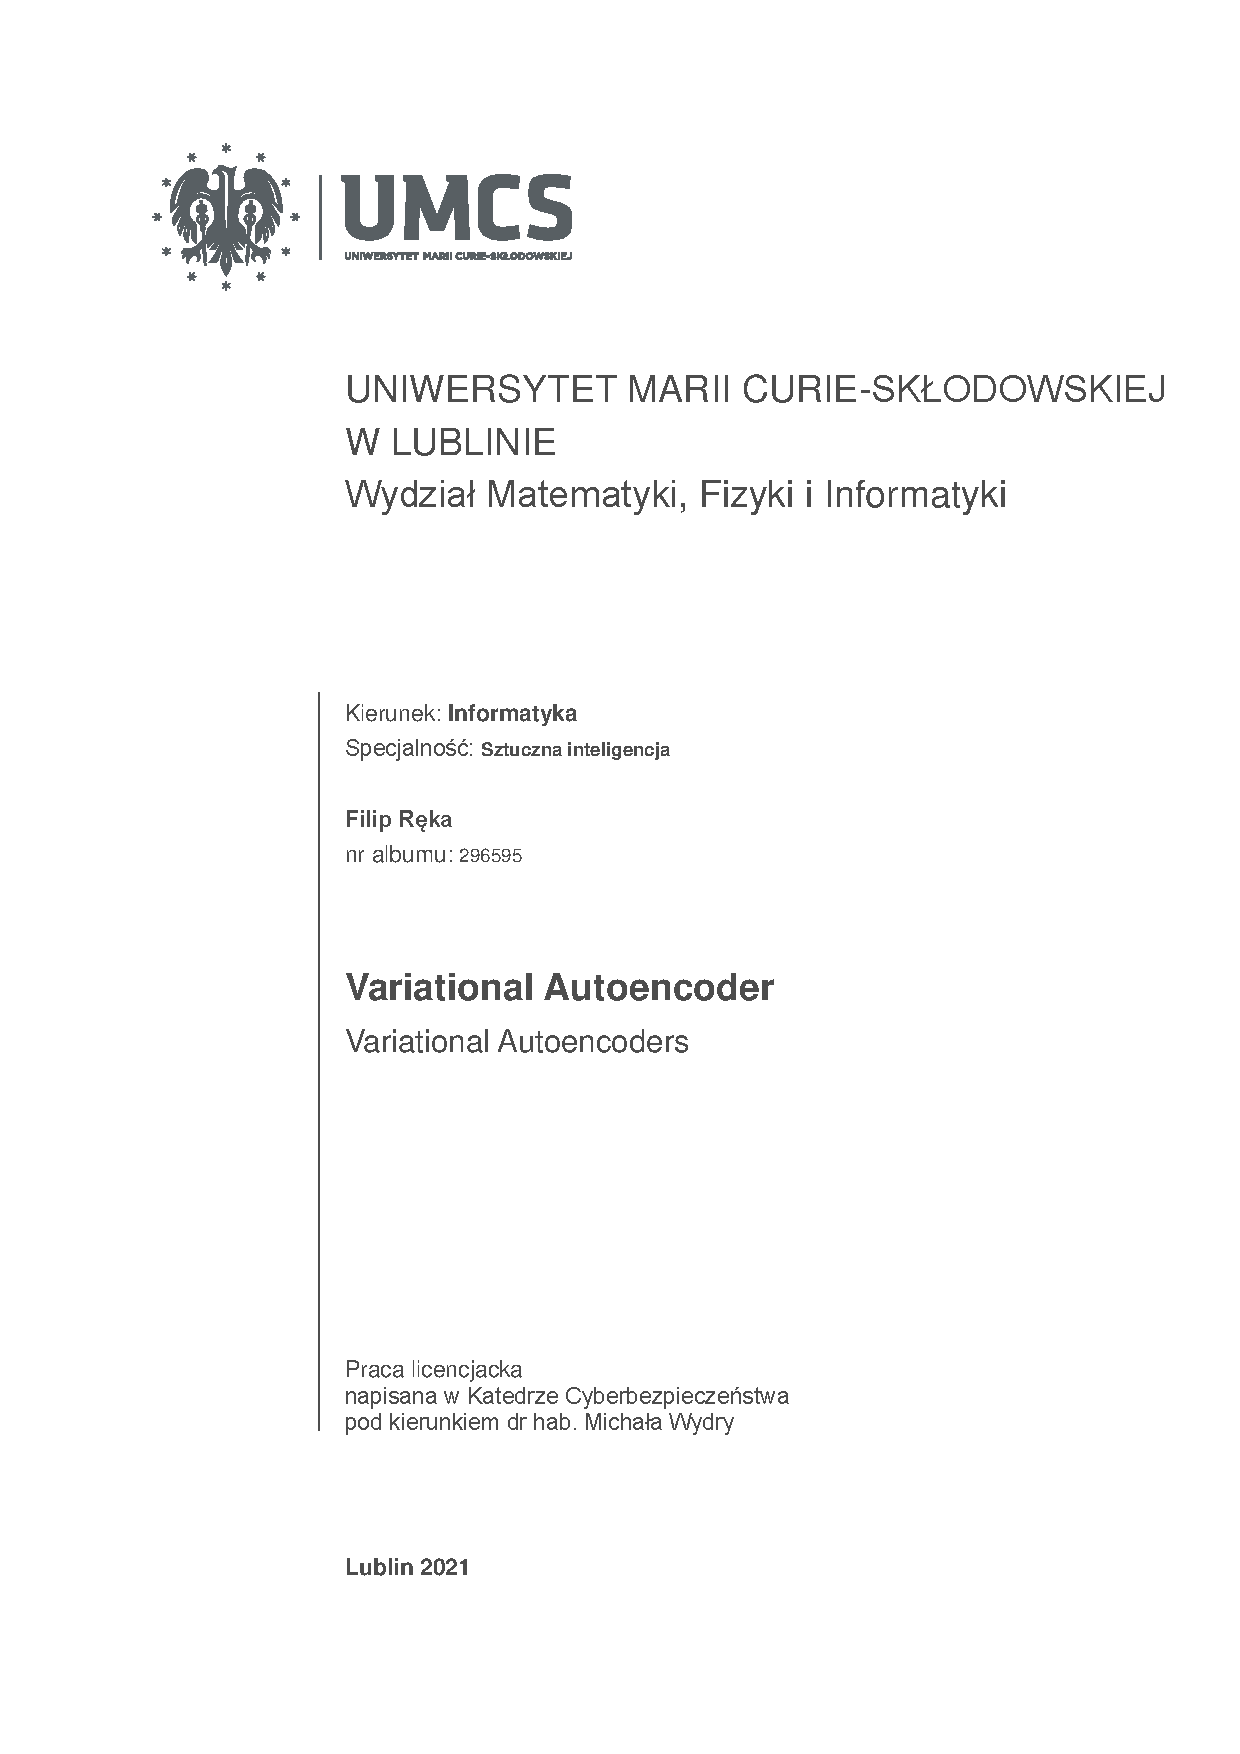
\includepdf{stronatytulowasvg}
% najpierw uzupełnij w 'stronatytulowa.odt' openoffice i wyeksportuj do 'stronatytulowa.pdf'

\newpage{}

\thispagestyle{empty}

\newpage{}



\tableofcontents{}

\chapter*{Wstęp} % z gwiazdką, więc bez numerka...
\addcontentsline{toc}{chapter}{Wstęp} % ...ale w spisie treści ma być

\chapter{Rozdział o czymś tam}

\section{Sekcja A}
\begin{itemize}
\item Siema siema co jest 5 \cite{cokolwiek}
\item siema co jest grane
\item koniec serio 
\end{itemize}

\lipsum[1-5]
\section{Sekcja B}
\subsection{podsekcja}
\label{podsekcjaaaaa121}

\lipsum[1-5]
\chapter{Rozdział o czymś innym}
Siema \cite{doersch2021tutorial}
\section{Sekcja C}
\lipsum[1-5]
\ref{podsekcjaaaaa121}
\section{Sekcja D}
\lipsum[1-5]

\chapter{Kolejny rozdział o niczym}
\section{Pozdrowienia do więzienia}
\lipsum[1]

\listoftables{} % jeśli są tabele
\addcontentsline{toc}{chapter}{Spis tabel}

\listoffigures{} % jeśli są tabele
\addcontentsline{toc}{chapter}{Spis rysunków}

\bibliographystyle{ieeetr}
\bibliography{./cytowania/cokolwiek.bib}


%\begin{thebibliography}{99}
%\addcontentsline{toc}{chapter}{Bibliografia}
% \bibitem aaaaaaaa
% \bibitem bbbbbbbb 
%\end{thebibliography}


\end{document}
